\begin{figure*}
\begin{centering}
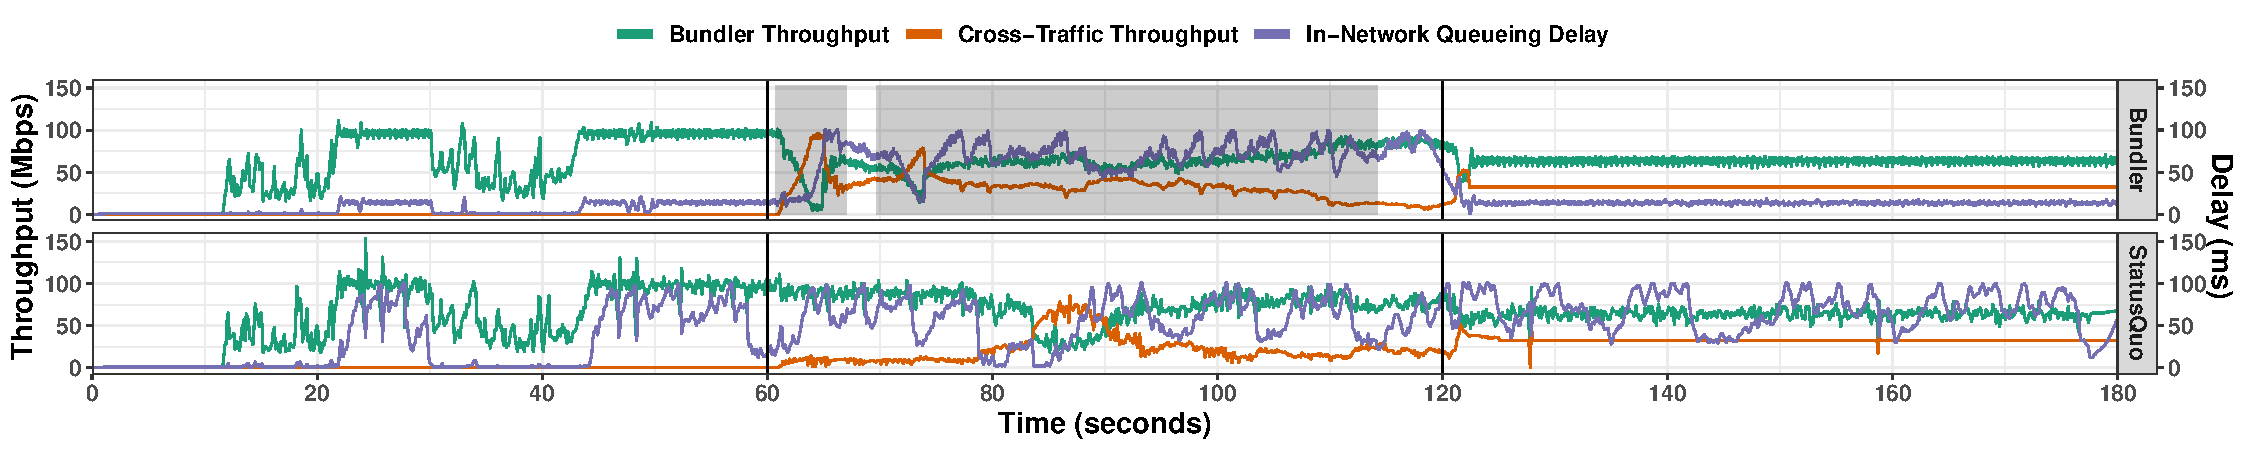
\includegraphics[width=\textwidth]{big_exp/timeseries}
\end{centering}
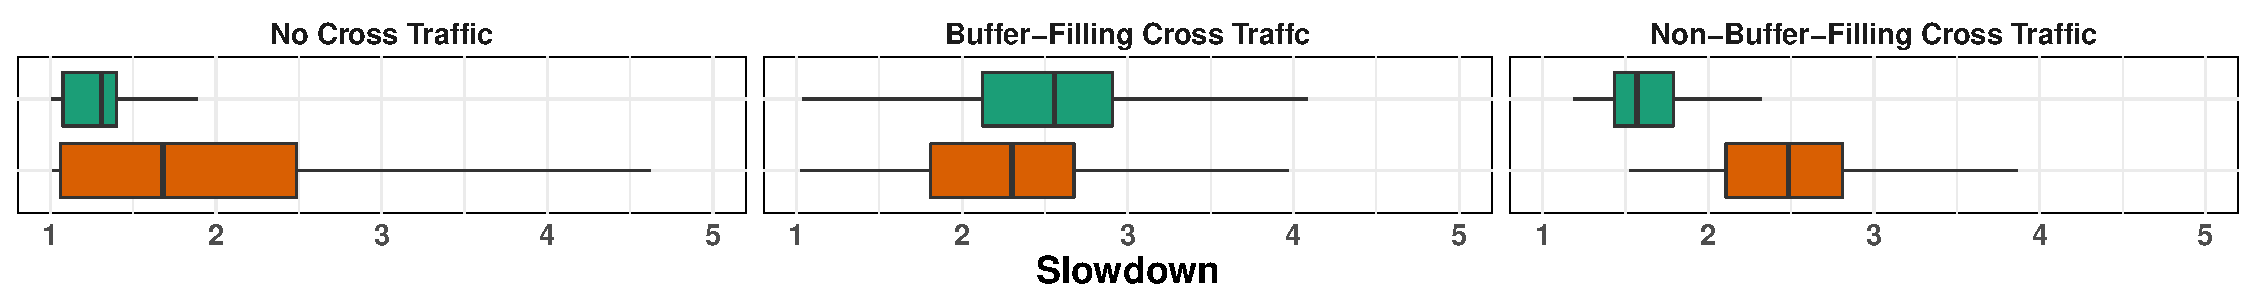
\includegraphics[width=0.95\textwidth]{big_exp/fcts}
\caption{\name's scheduling ability depends on the characteristics of the cross traffic over time. In this experiment, there are 3 periods: from 0 to 60 sec., there is no competing traffic, from 60 to 120 sec. there is buffer-filling cross traffic, and from 120 to 180 sec. there is non-buffer-filling cross traffic. The box-plots below each period show the distribution of short flow FCTs during that time. During the period with buffer-filling cross traffic, \name detects its presence and competes fairly. The shaded region indicates time \name spent in buffer-filling cross-traffic mode (\Sec{s:buffer-filling}).}\label{fig:eval:bigexp}
\end{figure*}
